\documentclass[margin,line]{resume}
\usepackage[hidelinks]{hyperref}
\usepackage{tikz}
\setlength{\textheight}{9.7in}
\newenvironment{absolutelynopagebreak}
{\par\nobreak\vfil\penalty0\vfilneg
\vtop\bgroup}
{\par\xdef\tpd{\the\prevdepth}\egroup
\prevdepth=\tpd}

\begin{document}
\begin{tikzpicture}
\clip (0,0) circle (1cm) ;
\node[anchor=center] at (0,0) {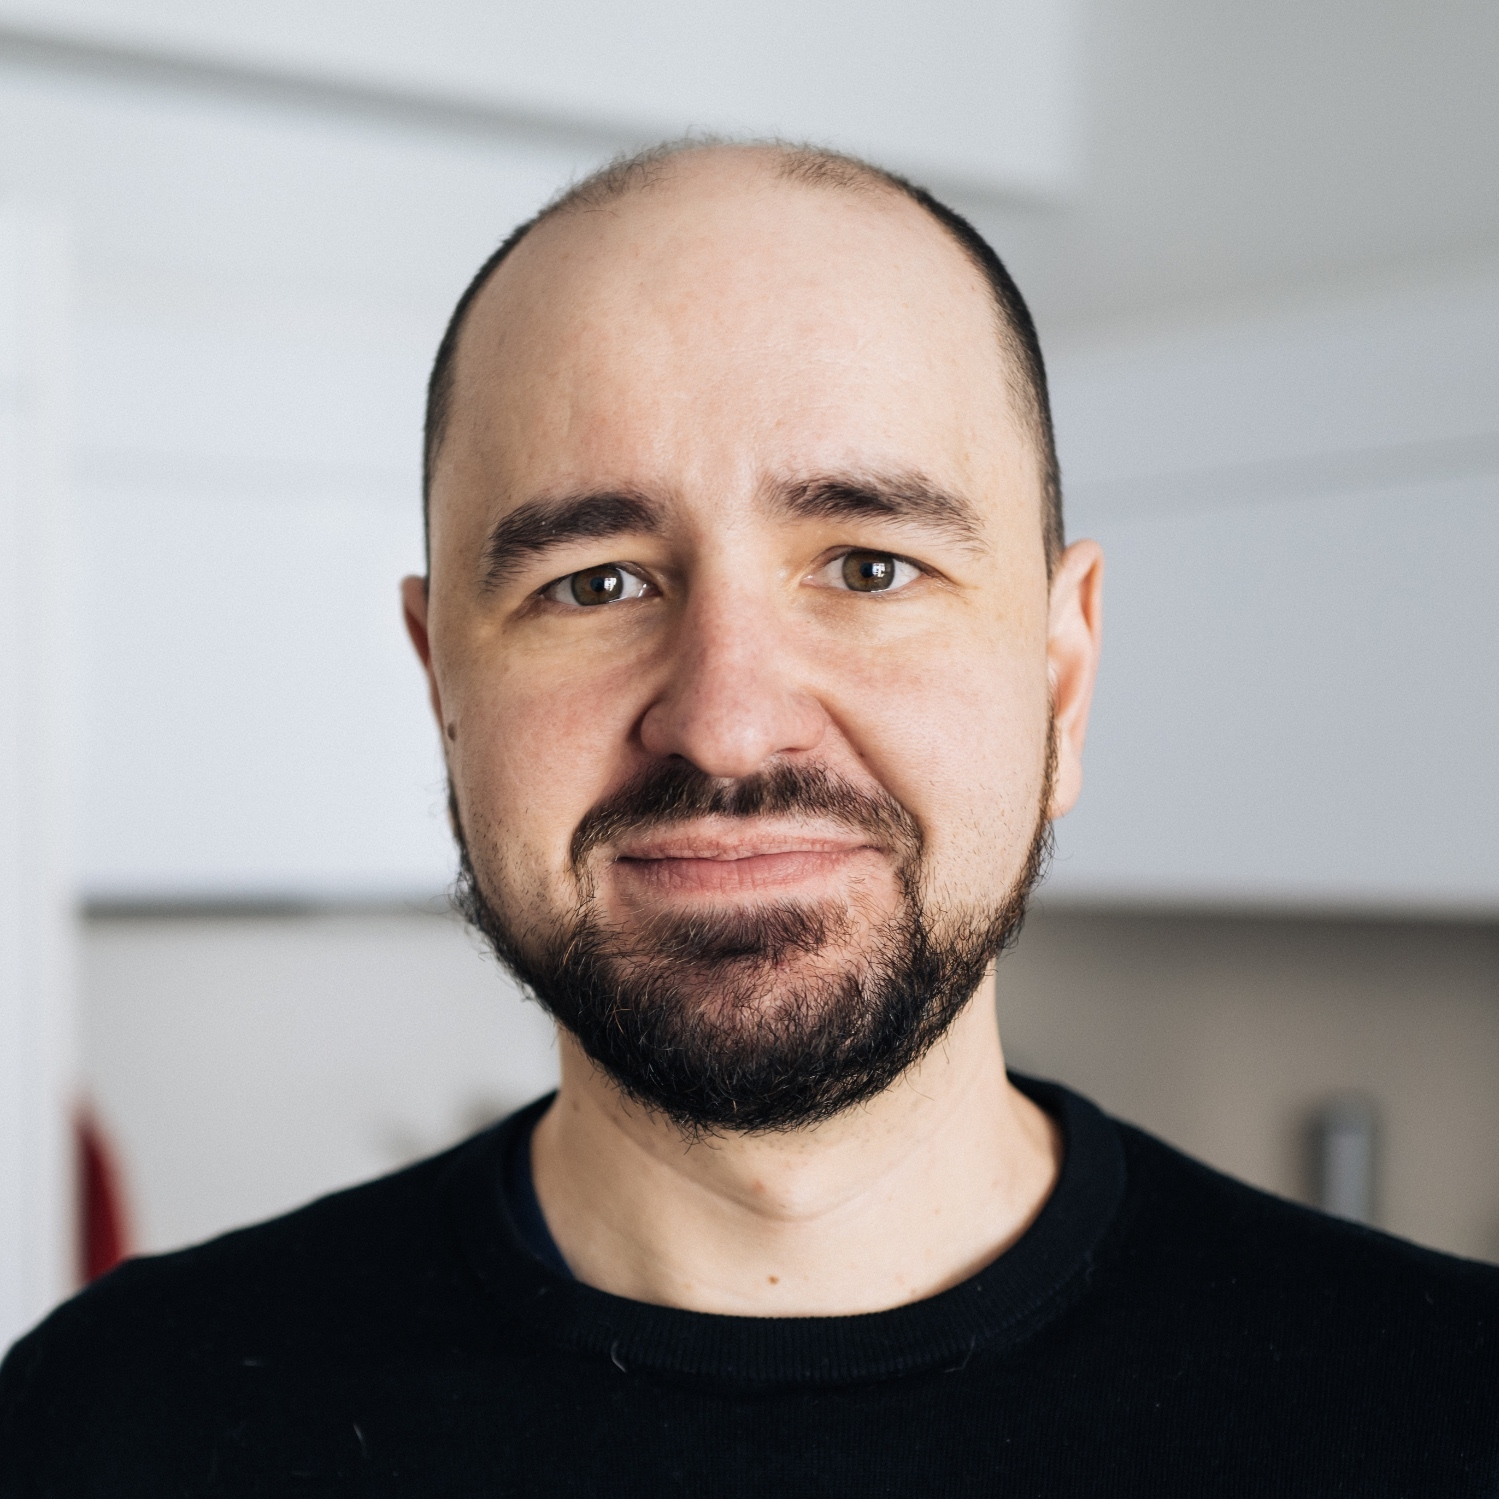
\includegraphics[width=2cm]{myface}};
\end{tikzpicture} \name{\Large Brenden Matthews}
\begin{resume}

\section{\mysidestyle Contact\\Information}

Email: \href{mailto:resume@brenden.brndn.io}{\texttt{resume@brenden.brndn.io}} \hfill
GitHub: \href{https://github.com/brndnmtthws}{\texttt{github.com/brndnmtthws}} \hfill
Website: \href{https://brndn.io}{\texttt{brndn.io}} \hfill
\vspace{3mm}

\section{\mysidestyle Professional\\Summary}

Experienced and accomplished software engineer with a strong background in Rust, C, C++, Python, and other programming languages. Recognized authority in the field of Rust programming with two highly acclaimed books published. Extensive experience in open source contributions and delivering impactful talks at prestigious conferences. Proven track record of successfully launching and managing businesses. Skilled in building and enhancing infrastructure using Kubernetes and other technologies. Strong leadership and consulting skills with a passion for driving innovation and delivering exceptional results.

\section{\mysidestyle Published\\Works}

\href{https://www.manning.com/books/code-like-a-pro-in-rust}{\textbf{Code Like a Pro in Rust}}, Manning Publications. ISBN 9781617299643.
\linebreak \href{https://www.manning.com/books/idiomatic-rust}{\textbf{Idiomatic Rust}}, Manning Publications. ISBN 9781633437463.

\vspace{3mm}

\section{\mysidestyle Public\\Speaking}

I have delivered numerous impactful talks on my work at prestigious conferences and private engagements, including renowned events such as \textbf{All Things Open}, \textbf{QCon}, \textbf{LinuxCon}, \textbf{ContainerCon}, and \textbf{MesosCon}.

\vspace{3mm}

\section{\mysidestyle Open\\Source}

I have made significant contributions to hundreds of influential open source projects, including well-known ones such as Apache Airflow, Apache Kafka, Apache Superset, Apache Spark, and Apache Mesos (where I am a PMC member). I am also proud to be a member of the esteemed Apache Software Foundation. Additionally, I have personally created several highly regarded projects, with a few notable ones highlighted below:

\href{https://github.com/brndnmtthws/conky}{\textbf{Conky}}, C and C++ \hfill \textbf{7.2k+ stars}\\
Conky is a highly versatile and widely used system monitor utility for UNIX systems.

\href{https://github.com/brndnmtthws/thetagang}{\textbf{ThetaGang}}, Python \hfill \textbf{2k+ stars}\\
ThetaGang is a cutting-edge equity options trading tool designed to capture premium from theta decay. It is specifically tailored for use with IBKR.

\href{https://github.com/brndnmtthws/dryoc}{\textbf{dryoc}}, Rust \hfill \textbf{270+ stars}\\
dryoc is a top-tier, pure-Rust general-purpose cryptography library that is fully compatible with libsodium. It boasts advanced features such as generic hash functions suitable for cryptography, protected memory, zeroization, and SIMD.

\vspace{3mm}

\begin{absolutelynopagebreak}
\section{\mysidestyle Professional\\Experience}

\textbf{Entrepreneur, Author, Consultant}, New York, NY\hfill \textbf{May 2019 -- present}\vspace{2mm}\\\vspace{1mm}%
\begin{itemize}
\item Successfully launched and managed multiple bootstrapped businesses
\item Provided expert consulting services to a diverse range of clients, delivering exceptional results
\item Authored two highly acclaimed books on Rust programming, establishing myself as a recognized authority in the field
\item Made significant contributions to numerous open source projects, further solidifying my reputation as a respected industry professional
\item Delivered captivating talks at various meetups, captivating audiences with my deep knowledge and expertise
\item Created a number of open source technology demonstration projects, showcasing my skills and expertise to a wide audience
\item Developed a comprehensive online training program for leetcoding in Rust based on the \emph{Cracking the Coding Interview} book, enabling students to learn from the comfort of their own home
\end{itemize}
\end{absolutelynopagebreak}

\vspace{5mm}

\begin{absolutelynopagebreak}
\textbf{Braze, Inc.}, New York, NY\hfill \textbf{Oct 2018 -- April 2019}\vspace{2mm}\\\vspace{1mm}%
\textsl{Engineering}

As a key member of the engineering team, I played a pivotal role in building and enhancing the infrastructure using Kubernetes.

\begin{itemize}
\item Led a highly successful initiative to transform ad-hoc Bash-based deployment scripts into a streamlined, declarative Helm and Terraform-based deployment system
\item Provided invaluable guidance and training to the entire engineering team, facilitating a seamless transition to Terraform and Helm
\item Successfully migrated the primary Rails monolith to Kubernetes, improving scalability and performance
\item Implemented a robust continuous integration and deployment system for Kubernetes applications, ensuring efficient and reliable software delivery
\item Developed a comprehensive monitoring and alerting system for Kubernetes applications, enabling real-time monitoring and alerting of critical issues
\item Spearheaded the development of a deployment pipeline for Kubernetes applications, significantly improving the efficiency and reliability of software delivery
\end{itemize}
\end{absolutelynopagebreak}

\vspace{5mm}

\begin{absolutelynopagebreak}
\textbf{Citadel LLC}, New York, NY\hfill \textbf{Oct 2017 -- Jun 2018}\vspace{2mm}\\\vspace{1mm}%
\textsl{Engineering}

As a member of the platform engineering group, I joined the data engineering team at Citadel to spearhead the development of their cutting-edge data platform technology. I primarily focused on integrating on-prem and cloud (AWS and GCE) data infrastructure.

\begin{itemize}
\item Led a highly successful initiative to modernize data access, control, and authorization, significantly enhancing data security and efficiency
\item Managed a seamless migration of legacy data systems to PostgreSQL on RDS backends, improving scalability and performance
\item Provided technical leadership to the data science team, guiding them on best practices for building and deploying large-scale machine learning jobs using Spark, Redshift, and Snowflake
\item Developed a comprehensive data governance strategy, ensuring compliance with industry regulations and best practices
\item Implemented a robust data quality monitoring system, enabling real-time monitoring and alerting of data quality issues
\end{itemize}
\end{absolutelynopagebreak}

\vspace{5mm}

\begin{absolutelynopagebreak}
\textbf{D2IQ (fka Mesosphere), Inc.}, San Francisco, CA\hfill \textbf{Jan 2015 -- Feb 2017}\vspace{2mm}\\\vspace{1mm}%
\textsl{Sales \& Engineering}

As one of the early employees at Mesosphere, I played a pivotal role in the company's foundation. I engaged in multiple customer engagements, serving in both pre-sales and post-sales positions. Additionally, I provided valuable assistance to management during fundraising pitches.

\begin{itemize}
\item Built and led the initial sales team, making key hires for VP Sales, early SEs, SAs, and Head of Services
\item Developed comprehensive cloud migration plans for enterprise customers, enabling them to leverage the power of container technology and accelerate their innovation
\item Delivered week-long in-depth onsite training sessions, equipping clients with the knowledge and skills to maximize the benefits of container technology
\item Advised C-level management at Fortune 500 companies on container technology adoption, helping them drive their digital transformation initiatives
\item Delivered captivating talks at various meetups and conferences, establishing myself as a thought leader in the industry
\item Contributed to various engineering efforts, leveraging my technical expertise to drive innovation and deliver exceptional solutions
\item Published several original blog posts, sharing my insights and experiences with a wide audience
\item Built and maintained marathon-lb, the canonical load balancing and service discovery tool for Marathon and DC/OS, further solidifying my reputation as a leading expert in the field
\end{itemize}
\end{absolutelynopagebreak}

\vspace{5mm}

\begin{absolutelynopagebreak}
\textbf{Airbnb, Inc.}, San Francisco, CA\hfill \textbf{Feb 2013 -- Jan 2015}\vspace{2mm}\\\vspace{1mm}%
\textsl{Engineering}

As one of the early employees at Airbnb, I joined the Data Infrastructure team to help scale the company's infrastructure and meet the growing demands of managing a large data warehouse. I collaborated closely with teams across the organization to fulfill their data needs and develop a robust set of data tooling.

\begin{itemize}
\item Spearheaded the development of the next generation of data infrastructure, leveraging open source tools such as Mesos, Hadoop, HDFS, Chronos, and Storm
\item Made significant contributions to several projects, including Mesos, Hadoop, Storm, Spark, Presto, Chronos, Marathon, and others
\item Played a key role in the early versions of Apache Superset (formerly known as Airpal), a powerful data exploration and visualization platform
\item Led the development of cutting-edge data processing tools, including Apache Airflow, enabling efficient and reliable data workflows
\item Implemented an automated verification system to improve data quality, ensuring the accuracy and reliability of Airbnb's data
\item Coined the team motto of \emph{"Provably correct data"}, emphasizing the importance of data accuracy and integrity
\item Delivered engaging internal tech talks on emerging technologies at Airbnb, sharing my knowledge and insights with colleagues
\end{itemize}
\end{absolutelynopagebreak}

\vspace{5mm}

\begin{absolutelynopagebreak}
\textbf{Newfield Wireless, Inc.}, Berkeley, CA\hfill \textbf{Sept 2009 -- Nov 2012}\vspace{2mm}\\\vspace{1mm}%
\textsl{Engineering}

At Newfield Wireless, I leveraged my expertise in 3GPP layer 3 to develop a highly efficient UMTS network data parser and indexer. I also designed and implemented a suite of real-time 3GPP LTE capture/parsing tools.

\begin{itemize}
\item Created a customized database solution with an integrated flexible query language, enabling real-time access to millions of streaming records
\item Designed and implemented an asynchronous communication library with C++ and Python interfaces, similar to ZeroMQ, to facilitate efficient and reliable communication
\item Developed a reporting library for generating key performance indicators from vast quantities of raw data, leveraging the customized database
\item Introduced new development and debugging methodologies to the team, significantly improving development speed and deliverable quality
\item Mentored and assisted junior and senior developers, fostering a collaborative and productive work environment
\item Oversaw the design and implementation of schema-based XML software specifications, ensuring adherence to industry standards
\end{itemize}
\end{absolutelynopagebreak}

\vspace{5mm}

\begin{absolutelynopagebreak}
\textbf{Real Time Measurements, Inc.}, Calgary, AB\hfill \textbf{2003 -- 2009}\vspace{2mm}\\\vspace{1mm}%
\textsl{Engineering}

\begin{itemize}
\item Developed end-user applications, web services, and embedded software, delivering high-quality solutions to meet customer needs
\item Played a key role in strategic planning, performance improvement, organizational design, e-commerce, new media, and Internet promotion, driving business growth and success
\item Planned and coordinated team-building exercises, demonstrating strong leadership skills and fostering a collaborative work environment
\item Configured and managed servers, automated backup systems, and provided exceptional customer and in-house support
\item Leveraged new technologies to enhance the product-to-customer experience, delivering timely and cost-effective solutions
\item Implemented a cost reduction IT strategy, optimizing existing infrastructure and minimizing the need for additional equipment purchases
\end{itemize}
\end{absolutelynopagebreak}

\vspace{3mm}

\section{\mysidestyle Programming\\Experience}

\emph{Languages:} Rust, C, C++, Python, Ruby, Bash, Go, Java, Scala, Kotlin, \LaTeX \\
\emph{Data Technology:} Kafka, Cassandra, Redis, PostgreSQL, ElasticSearch/Lucene, MySQL, Hadoop, Hive, Presto, RedShift, BigQuery, SQS, EMR, RDS, Snowflake, PyTorch, TensorFlow

\section{\mysidestyle Authentication}

The original source for this resume is available at
\href{https://github.com/brndnmtthws/resume}{\texttt{github.com/brndnmtthws/resume}}.
Use the contact email address at the top of this document or the one listed
on my GitHub profile if you suspect shenanigans (such as fake candidates
posing with my profile/details).
\end{resume}
\end{document}
